% !Mode:: "TeX:UTF-8"

\chapter{绪论}
\section{研究背景及意义}

魔方作为凝聚了人类智慧的玩具,不仅可以培养人们的空间想象力、记忆力等,更可以锻炼手脑协同工作能力,其还原过程代表着人类三维空间想象及逻辑推理运算等方面的智力行为~\cite{1}~\cite{2}。再者,如今出现以不同方式还原魔方的竞技运动,例如单手还原魔方、双手还原魔方等。可见在解魔方这个过程中,人们有各式各样的办法与招式。而标准三阶魔方可称得上是所有魔方类型中的经典。如下图~\ref{fig:1-1}~是一个标准的三阶魔方实例图。

\begin{figure}[H]
	\centering
	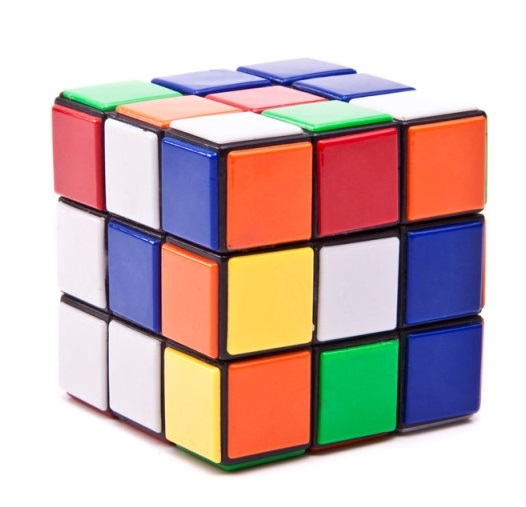
\includegraphics[width=0.4\textwidth]{1-1}
	\caption{标准三阶魔方}\label{fig:1-1}
\end{figure}

近年来,研究人员开始考虑研究魔方还原的机器人自动化设备以追求魔方复原速度上的极致。对于魔方还原的机器人自动化设备,其技术关键是如何设计复原操作装置、颜色识别算法以及魔方复原算法来可靠地完成复原任务。这正是本论文研究所需要解决的问题。本论文借助Arduino嵌入式系统开发魔方还原系统~\cite{3}~\cite{4},不仅可以极大地简化开发步骤,而且能够提高还原效率。本系统经过复杂的计算与推理,寻找还原步骤简化规律,可快速建立最优的还原操作;同时依次通过颜色识别模块、还原求解模块、串口通讯模块和电机转动模块可实现对任意打乱状态下的魔方进行精准、快速地还原。

\section{国内外研究现状}

早在1978年,匈牙利的数学家们把魔方介绍给当年国际数学家代表会的专家学者,这是魔方在数学家面前的首次正式亮相,同时也引起了极大的反响,受到了人们的广泛关注。
在随后的一段时间里英国便出现了历史上第一批的魔方理论研究小组。在1981年3月,魔方首次登上了《科学美国人》的封面。在魔方领域的众多概念中,魔方复原所需的最小转动次数称为“上帝之数”,也就是至少需要经过多少旋转操作能够复原一个打乱的魔方~\cite{1}。
“上帝之数”的具体数值吸引了非常多的魔方研究者~\cite{5},其中有相当一部分是数学家。数学家们用几十年的研究证明,任何打乱都可以在二十步内解决,即上帝之数为二十~\cite{6}。

近年来,魔方复原系统机器人引起了国内外研究人员的广泛兴趣。在国外,最早出现的魔方复原系统是在2010年世界制造者博览会上展出的名为“The Cubinator”的双臂魔方还原机器人,这款机器人是皮特-雷蒙德设计的,其工作原理是由相互垂直、呈九十度角的两个机械手臂旋转配合,通过一系列机械手臂对魔方的松紧操作,从而完成魔方复原。2011年,斯威本科技大学的一个学生小组研制了一款名为Ruby的魔方复原机器人,被人们誉为“最快魔方机械手”,该魔方机器人以10.96 s的成绩打破当时机器人复原魔方的最快纪录。2014年,由ARM的两位工程师完成的CubeStormer3机器人还原魔方仅需3.253秒,而上一代产品CubeStormer2需要5.27秒,并且当时人类复原魔方的记录则为5.5秒,机器人复原魔方的水平已远远领先人类的水平,该机器人的旋转部分采用的是四个与乐高机器人配对的伺服电机,机器人采用ARM驱动的三星Galaxy S4智能手机,由三星Exynos 5 Octa应用处理器驱动,分析立方体,并指导四个机器人手进行旋转操作,ARM9处理器还为八块乐高 MINDSTORMS EV3积木提供动力,执行电机排序和控制。2019年,日本工程师Human Controller制作了一款自还原的魔方,该工程师把魔方内部“魔改”了一番,把原本是简单连接杆的核心改成了电子机械结构~\cite{7},其结构包含了电机、电线、电池等复杂机械结构,使得魔方拥有了自动化的基础,魔方在被打乱的过程中,其内部芯片会存储打乱的顺序,当魔方检测到一段时间没有发生人为转动时,则会自动开始按照打乱的顺序倒序进行相反方向旋转的操作。除此之外,随着科技水平的进步,德国工程师Albert Beer设计的名为“Sub 1 Reloaded”的魔方机器人是目前世界上魔方复原速度最快的机器人,能够在 0.637 秒的时间内完成任务,其主要结构为空间中相互垂直的6个旋转轴,该魔方机器人通过两张照片来识别魔方的色块样式,然后借助 Herbert Kociemba 发明的两阶段算法~\cite{8}来计算出一套解决方案,最终在英飞凌处理器的指挥下,让机械臂在1s内完成最后的操作。相比于文献\mycite{9}中介绍的魔方复原的算法,两阶段算法具有在复原步骤上有很明显的优势。

在国内,也有许多魔方爱好者设计了不同复原方式的魔方复原系统,例如用双臂解魔方机器人系统~\cite{10}~\cite{11}、四臂魔方还原系统~\cite{12}等,除此之外还有基于不同嵌入式平台的系统~\cite{13},例如基于FPGA异构平台的魔方还原系统~\cite{14}、基于ARM9的魔方机器人系统~\cite{15}、基于STM32的解魔方系统~\cite{11}~\cite{16}等。南通理工学院的解魔方机器人~\cite{17}可以在七十秒之内完成魔方的复原。北京理工大学珠海学院自动化学院设计的魔方还原系统采用双气动控制的方法,其魔方还原成功率可达到97\%~\cite{10}。济南大学的田田~\cite{18}~\cite{19}设计了一款同样基于气动的解魔方组合机械手,该方法通过采用带有CMOS图像传感器的摄像头来捕获各个魔方块的颜色图像,再通过RGB颜色模型完成魔方色块的颜色识别,以本地计算机为上位机,采用Thistlethwaite算法计算出复原步骤,最后通过控制气动机械手进行魔方复原。大连民族学院的董海洋~\cite{20}设计了一款通过四轴还原魔方的类人机械臂机器人,以安卓操作系统的智能机作为上位机,通过摄像头完成图像采集,并计算出还原指令,通过嵌入式控制板连接舵机,再接收客户端发出的还原指令,最终串行调度相互垂直的四个机械手臂,从而执行魔方复原动作。东北大学的张雪娇~\cite{21}设计了一款硬件部分由乐高组件组成的魔方机器人,该机器人采用能将光学影像转化为数字信号的CCD半导体作为图像采集模块,并使用笔记本电脑作为上位机对捕捉到的图像进行预处理与魔方块颜色识别。除此之外,国产魔方品牌GAN设计的全球消费级智能魔方机器人GAN Robot能在五秒内复原任意打乱的魔方。该机器人采用的是五轴伺服系统,由动力台、动力臂及X旋爪组成,四向卡位底座,固定动力臂。若要进行复原操作,则需要使用配套的魔方,并且在相应的APP平台上,其复原的原理是魔方中心轴记录打乱的顺序并通过蓝牙将其顺序发送到APP平台上,通过APP平台进行还原算法的推理,得出还原的顺序及各自的转动方向后将其发送到四向卡位底座进行还原。

随着上述各种魔方还原机器人的出现,也有越来越多的各界人士包括数学家们研究魔方还原算法,追求魔方还原在速度、效率上的极致。并且由于解魔方本身具有趣味性及可观赏性,研究解魔方的人也越来越多。

\section{本文的主要工作}

本文主要的研究目标是基于Arduino单片机设计并实现一款三阶魔方的复原系统。在开发本系统的前期准备工作中需要对系统的整体硬件框架进行三维建模,并深入学习研究Kociemba提出的两阶段算法。系统的建模工作完成后,便需要开始系统的编码工作。通过上下位机的串口通信实现上位机的指令发送以及下位机的指令接收。在上位机编程中包含结合QT进行可视化界面设计等部分。本文阐述具体的研究工作主要包括以下几个方面:

(1)对魔方系统的硬件框架建模并搭建。考虑到本系统结合软硬件协同设计,并且为了硬件框架搭建的可行、有效,因此需要借助三维建模对系统的每一个零部件进行精确设计。建模完毕后方可实际搭建该系统。

(2)深入研究魔方复原的两阶段算法,提高魔方复原的效率。首先确定当下主流的魔方复原算法,再对比不同算法间的优缺点,选择最适合本课题系统的魔方复原算法。待确定算法后,再深入理解算法其中的数学原理及操作步骤,确定算法中不同阶段的输入输出从而进一步对算法进行微调。

(3)上位机编程。使用Python语言在上位机编写程序。其中包括可视化界面设计部分,魔方块颜色识别部分,串口通信部分,人机交互部分等。在每次识别魔方块颜色后,为防止小概率识别错误的发生,另外还增加魔方块颜色纠错功能。待复原算法得出还原步骤及顺序后,再通过串口将指令发送至下位机,进而驱动电机带动魔方面旋转。

(4)下位机编程。该部分的主要工作是将上位机发送的魔方复原解法转换成电机的转动操作。针对不同指令,电机进行不同的旋转操作。通过下位机编程能有效、迅速地将上位机的复原解法传递至电机部分。此外在这一部分中,系统还实现了部分并行还原的算法,可进一步缩小还原操作的用时。

(5)系统测试。在所有工作基本完成后,需要对系统进行大量测试。主要目的是发现系统中隐藏的一些难以被发现的问题。通过测试才能发现一些在实现本系统时忽略的问题。

在本课题初期的资料查阅阶段,通过阅读大量中、英文文献综述发现,从魔方被发明至今的时间里,魔方复原领域的研究者们产出了大量的成果,设计并实现了许多速度快、效率高、复杂度低的算法~\cite{22},这些算法相较传统方法都有巨大的提升。但是结合本课题在魔方复原系统方向的实际需求,仍有以下难点等待后续工作的解决:

1)针对不同光照环境下的魔方块颜色识别方面的性能有待提升。现有研究的普遍特点是基于摄像头对魔方颜色块进行识别,大部分现有研究并不能摆脱对摄像头的依赖,但是摄像头对图片颜色的识别又受光照等环境因素的影响。因此,如何在不同的环境因素的影响下能稳定识别魔方块的颜色是本课题的重要技术难点。

2)魔方复原算法需要进一步改进。本课题拟采用Kociemba提出的两阶段算法,针对任意打乱状态的魔方都可在二十步内得到解法。现有的算法~\cite{23}仍存在一些问题,特别是在转动操作十分单一的时候,此时该算法得到的结果并不是真正意义上的最优解。

3)电机与魔方中心块的契合。就目前资料来看,有一部分魔方系统是采用3D打印技术打印出将魔方中心块与电机相连接的零部件,而也有一部分魔方系统是使用类似夹子的工具将单个魔方面夹紧进行旋转。不同的策略所导致魔方旋转的速度也大不相同。因此在电机与魔方中心块连接的设计部分,也是该方向的难点之一。

\section{本文的创新点}

1.	在硬件结构方面,本论文提出的基于闭环步进电机的六轴复原架构采用电机与魔方中心块一对一紧扣的设计,使得每个魔方面的旋转操作由单个电机负责,不再出现多个旋转操作的结果最后只是旋转一个面的现象,从而极大程度上提升魔方复原效率。相比于二轴、四轴等魔方复原系统,该架构的翻动操作更加灵活迅速、更具稳定性,在还原速度上具有根本的优势。

2.	在现阶段还原步骤最少的Kociemba魔方复原算法的基础上提出了并行还原优化算法,将魔方复原步骤序列中存在互不干扰的对立面旋转操作并行化,既不影响魔方复原序列,也能减少魔方复原的总步骤数,可进一步缩短魔方复原的时间。测试结果表明,与串行复原相比,使用并行还原优化算法的效果十分显著。

\section{本文的组织结构}

本文一共分为以下四个章节,各章具体内容如下所示:

第一章简要介绍魔方复原系统的研究背景,综合对比国内外研究现状及成果的优缺点,并对现有魔方还原系统进行分析与简要归类判断,除此之外还介绍了本文的主要工作和组织架构。

第二章首先介绍在硬件层面开发本魔方复原系统所应用到的设备等相关内容。紧接着介绍了自主设计的PCB电路板,其目的是追求高度集成化,同时也为上、下位机通信打下硬件基础。最后列举展示在计算机中设计的三维建模仿真与实际搭建后的结果图。

第三章首先是简要介绍了在软件层面开发魔方复原系统的所涉及到的操作系统,集成开发环境以及部分重要模块,接着从数学的群论角度~\cite{24}~\cite{25}出发详细说明了两阶段算法的原理及实现步骤,再接着提出通过并行的旋转操作对还原算法进行进一步优化的想法,最后列举系统中已有的功能并附上截图加以文字说明。

第四章选取了本系统的部分模块进行对比实验。实验表明,本系统使用的魔方块颜色识别算法、复原算法及并行算法均可有效提高系统复原魔方的速度。

第五章对本篇文章的所有内容进行总结,针对本系统现有功能的不足提出问题以及列举下一步的改进工作。

\section{本章小结}

本章简要阐述了基于Arduino的三阶魔方复原系统研究的意义以及目前国内外本领域已有的一些研究成果,并介绍了本研究课题的主要工作以及技术难点,本章的最后列举了本篇论文的组织架构。